%%%%%%%%%%%%%%%%%%%%%%%%%%%%%%%%%%%%%%%%%%%%%%%%%%%%%%%%%%%%%%%
%
%
%%%%%%%%%%%%%%%%%%%%%%%%%%%%%%%%%%%%%%%%%%%%%%%%%%%%%%%%%%%%%%%

\documentclass{article}
\usepackage{graphicx}
\usepackage{fullpage}

\title{Übungsblatt 2}
\author{Tobias Baake (247074), Dylan Ellinger (247316), Nikiforos Tompoulidis (247714)}
\begin{document}
\maketitle

\section{Aufgabe CSG}
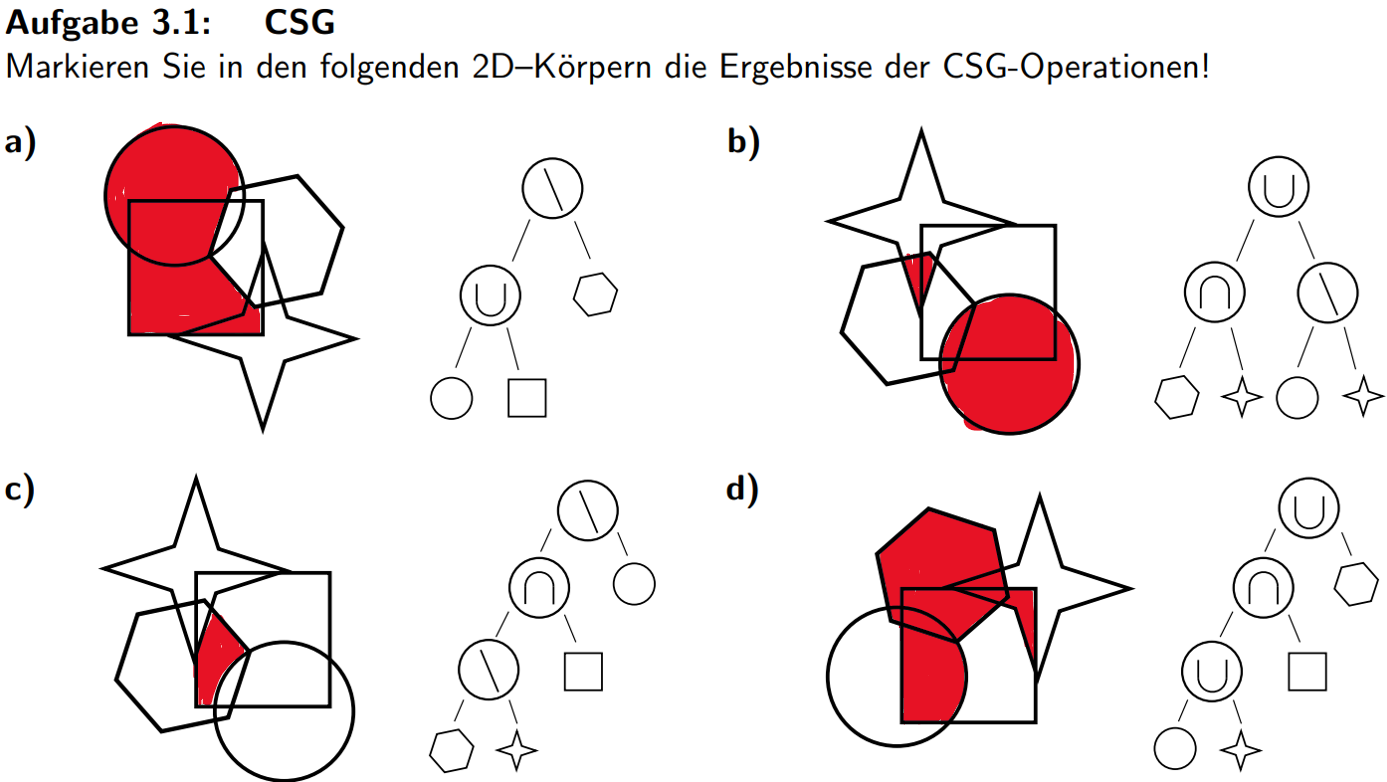
\includegraphics[width=400pt]{./files/Übung3.1.png}

\section{Aufgabe Quadtrees}
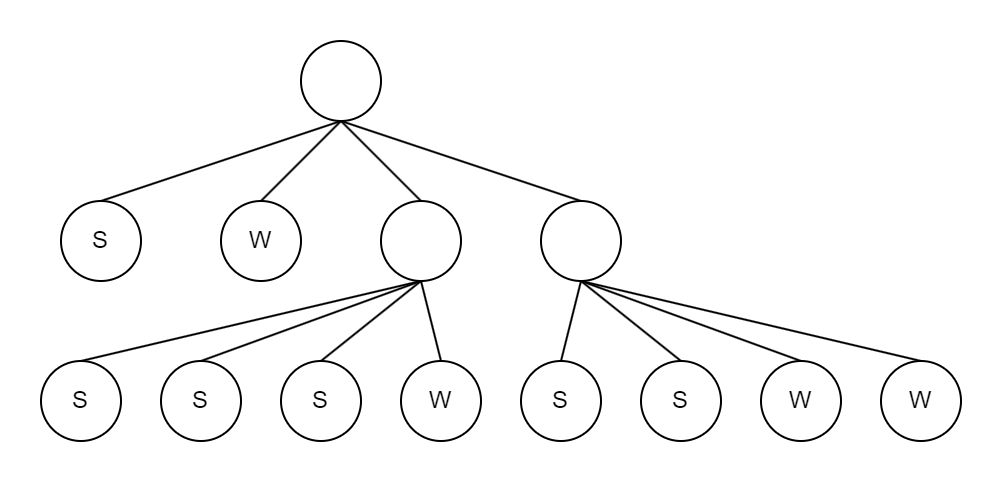
\includegraphics[width=400pt]{./files/Übung3.2.drawio.png}

\section{Aufgabe Bézierkurzen}

\emph{a)}
keine kubische Bezierkurve, weil die Form der Kurve 5 bezierpunkte impliziert, aber nur 4 gegeben sind, weswegen die Kurve eher wier ein "S" aussehen müsste.
\\
\emph{b)}
kubische Bezierkurve, mit mehr gewsichtung auf Punkt $b_1$.
\\
\emph{c)}
kubische Bezierkurve, mit Gewichtung auf $b_1$ und $b_2$.
\\
\emph{d)}
keine kubische Bezierkurve, weil die Gewichtung von $b_1$ und $b_2$ in der Kurve falsch herum dargestellt ist.
\\
\emph{e)}
kubische Bezierkurve, weile alle Punke in einer Gerade liegen, und somit die Kurve auch eine Gerade ist.
\\
\emph{f)}
keine kubische Bezierkurve, denn die "Beulen" der Kurve müssten andersherum sein, damit die Gewichtung/Richtung der Punkte stimmt.

\end{document}

